\documentclass[10pt,xcolor={dvipsnames}]{beamer}
\usetheme[progressbar=frametitle]{PaloAlto}
\usepackage{appendixnumberbeamer}
\usepackage{booktabs}
\usepackage[scale=2]{ccicons}
\usepackage{pgfplots}
\usepgfplotslibrary{dateplot}
\usepackage[utf8]{inputenc}
\usepackage{fancyvrb}
\usepackage{xspace}
\newcommand\tab[1][1cm]{\hspace*{#1}}
\usepackage{pgf-pie}
\usepackage{color}

\title{Proyecto 1}
\subtitle{Un generador de Scanners}
\date{}
\author{
    José Ceciliano Granados\newline 2016087245
    \newline \newline
    Audra Rodríguez Mora \newline 2015101893
    \newline \newline
    David Valverde Zuñiga \newline 200922986
}
\institute{Instituto Tecnológico de Costa Rica
    \newline Compiladores e Intérpretes
    \newline I Semestre 2019 }
}

\begin{document}

    \maketitle

    \section{Introducción}
        \begin{frame}[fragile]{Introducción}
        \begin{alertblock}{Introducción}
                Flex es una herramienta de análisis lexico desarrollada para la generación de Scanners, programas que reconocen patrones léxicos en el texto.\\
                Su nombre significa "fast lexical analyzer generator" y se encarga de leer las entradas recibidas para generar la descripción de un scanner en forma de pares de expresiones regulares y código C, llamadas "reglas".\\

        \end{alertblock}
        \end{frame}

    \section{Scanning}
        \begin{frame}[fragile]{Scanning}
            \begin{alertblock}{Scanning}
                Mediante proceso de Scanning se identifican los diferentes lexemas de un lenguaje. Flex genera como salida un archivo C que define una rutina en específico, que junto con una biblioteca genera un ejecutable con la capacidad de analizar su entrada para la aparición de expresiones regulares. Cada vez que encuentra una, ejecuta el código C correspondiente.\\
                Todo esto se puede traducir a que Flex es capaz de crear un "Deterministic Finite Automaton" (DFA) que se utilizará para adquirir los diferentes lexemas que se pretenden escánear.
            \end{alertblock}
        \end{frame}


    \section{Gráficos}
        \begin{frame}[fragile,allowframebreaks]{Histograma}
        \begin{alertblock}{Histograma}
            A continuación se presenta un histograma que muestra la cantidad de cada tipo de \textit{token} encontrado en el código fuente:
            \end{alertblock}
        \end{frame}

    \subsection{Gráfico Barras}
        \begin{frame}[fragile]{Histograma} 
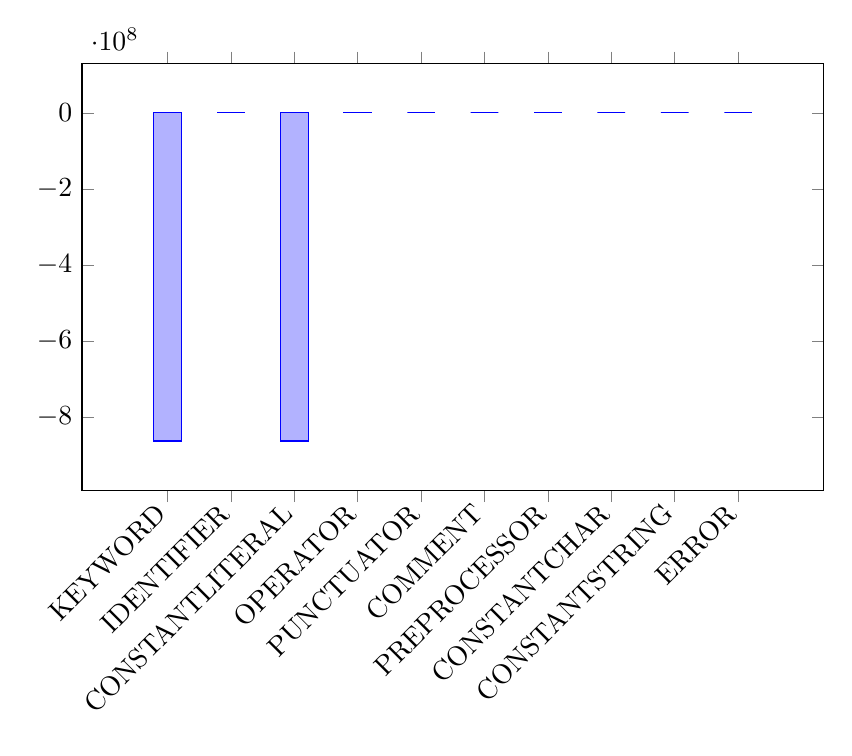
\begin{tikzpicture}     
\begin{axis}[ybar, enlargelimits=0.15, x tick label style={rotate=45, anchor=east},    symbolic x coords={KEYWORD, 
IDENTIFIER, 
CONSTANTLITERAL, 
OPERATOR, 
PUNCTUATOR, 
COMMENT, 
PREPROCESSOR, 
CONSTANTCHAR, 
CONSTANTSTRING, 
ERROR, 
},xtick=data,width=11cm,height=7cm] 
 \addplot coordinates {(KEYWORD,-863060829) 
(IDENTIFIER,32722) 
(CONSTANTLITERAL,-863060830) 
(OPERATOR,32716) 
(PUNCTUATOR,15) 
(COMMENT,0) 
(PREPROCESSOR,0) 
(CONSTANTCHAR,0) 
(CONSTANTSTRING,0) 
(ERROR,0) 
};
\end{axis}  
\end{tikzpicture} 
\end{frame}
    \subsection{Gráfico Pastel}
        \begin{frame}[fragile]{Histograma} 
\begin{tikzpicture} 
\pie[text=legend]{ 7/KEYWORD, 18/IDENTIFIER, 7/CONSTANTLITERAL, 7/OPERATOR, 47/PUNCTUATOR, 5/COMMENT, 0/PREPROCESSOR, 0/CONSTANTCHAR, 7/CONSTANTSTRING, 0/ERROR, }
\end{tikzpicture}
\end{frame}

  \section{Errores}
      \begin{frame}[fragile,allowframebreaks]{Histograma}
      TSource.in: In function ‘main’:
TSource.in:15:10: alerta: declaración implícita de la función ‘printf’ 
   printf(a);
        ^

TSource.in:16:15: Error de sintaxis:  declaración esperada o declaración al final de la entrada

              ^



Compilacion terminada con 1 errores.

      \end{frame}


    \section{Analisis Léxico}
        \begin{frame}[fragile,allowframebreaks]{Analisis Léxico}
        \begin{alertblock}{Codigo fuente}
            A continuación se presenta el código fuente con colores demostrando la división de \textit{tokens}.
            \end{alertblock}
        \end{frame}

        \begin{frame}[fragile,allowframebreaks]{Resaltado de sintaxis}~\newline\newline\color{Sepia}\verb$int$ \color{BlueViolet}\verb$FUNCION$\color{OliveGreen}\verb$($\color{OliveGreen}\verb$)$ \color{OliveGreen}\verb${$\newline \color{Sepia}\verb$int$ \color{BlueViolet}\verb$a$ \color{OliveGreen}\verb$=$ \color{BurntOrange}\verb$3$\color{OliveGreen}\verb$;$\newline \color{Sepia}\verb$return$ \color{BlueViolet}\verb$a$\color{OliveGreen}\verb$;$\newline\color{OliveGreen}\verb$}$\newline\newline\newline\color{Sepia}\verb$int$ \color{BlueViolet}\verb$main$\color{OliveGreen}\verb$($\color{OliveGreen}\verb$)$\color{OliveGreen}\verb${$\newline    \newline    \color{BlueViolet}\verb$FUNCION$\color{OliveGreen}\verb$($\color{OliveGreen}\verb$)$\color{OliveGreen}\verb$;$\newline    \color{Sepia}\verb$int$ \color{BlueViolet}\verb$a$ \color{OliveGreen}\verb$=$ \color{BurntOrange}\verb$9$\color{OliveGreen}\verb$;$\newline    \color{BlueViolet}\verb$a$ \color{ProcessBlue}\verb$+$\color{OliveGreen}\verb$=$ \color{BurntOrange}\verb$7$\color{OliveGreen}\verb$;$\newline\newline\newline    \color{BlueViolet}\verb$printf$\color{OliveGreen}\verb$($\color{BlueViolet}\verb$a$\color{OliveGreen}\verb$)$\color{OliveGreen}\verb$;$\newline\color{OliveGreen}\verb$}$\newline
\end{frame}



\end{document}
